%% bare_conf.tex
%% V1.4b
%% 2015/08/26
%% by Michael Shell
%% See:
%% http://www.michaelshell.org/
%% for current contact information.
%%
%% This is a skeleton file demonstrating the use of IEEEtran.cls
%% (requires IEEEtran.cls version 1.8b or later) with an IEEE
%% conference paper.
%%
%% Support sites:
%% http://www.michaelshell.org/tex/ieeetran/
%% http://www.ctan.org/pkg/ieeetran
%% and
%% http://www.ieee.org/

%%*************************************************************************
%% Legal Notice:
%% This code is offered as-is without any warranty either expressed or
%% implied; without even the implied warranty of MERCHANTABILITY or
%% FITNESS FOR A PARTICULAR PURPOSE! 
%% User assumes all risk.
%% In no event shall the IEEE or any contributor to this code be liable for
%% any damages or losses, including, but not limited to, incidental,
%% consequential, or any other damages, resulting from the use or misuse
%% of any information contained here.
%%
%% All comments are the opinions of their respective authors and are not
%% necessarily endorsed by the IEEE.
%%
%% This work is distributed under the LaTeX Project Public License (LPPL)
%% ( http://www.latex-project.org/ ) version 1.3, and may be freely used,
%% distributed and modified. A copy of the LPPL, version 1.3, is included
%% in the base LaTeX documentation of all distributions of LaTeX released
%% 2003/12/01 or later.
%% Retain all contribution notices and credits.
%% ** Modified files should be clearly indicated as such, including  **
%% ** renaming them and changing author support contact information. **
%%*************************************************************************


% *** Authors should verify (and, if needed, correct) their LaTeX system  ***
% *** with the testflow diagnostic prior to trusting their LaTeX platform ***
% *** with production work. The IEEE's font choices and paper sizes can   ***
% *** trigger bugs that do not appear when using other class files.       ***                          ***
% The testflow support page is at:
% http://www.michaelshell.org/tex/testflow/



\documentclass[conference]{IEEEtran}
\usepackage{url}
\usepackage{graphicx}
\graphicspath{ {images/} }

%
\ifCLASSINFOpdf
  % \usepackage[pdftex]{graphicx}
  % declare the path(s) where your graphic files are
  % \graphicspath{{../pdf/}{../jpeg/}}
  % and their extensions so you won't have to specify these with
  % every instance of \includegraphics
  % \DeclareGraphicsExtensions{.pdf,.jpeg,.png}
\else
  % or other class option (dvipsone, dvipdf, if not using dvips). graphicx
  % will default to the driver specified in the system graphics.cfg if no
  % driver is specified.
  % \usepackage[dvips]{graphicx}
  % declare the path(s) where your graphic files are
  % \graphicspath{{../eps/}}
  % and their extensions so you won't have to specify these with
  % every instance of \includegraphics
  % \DeclareGraphicsExtensions{.eps}
\fi



% correct bad hyphenation here
\hyphenation{op-tical net-works semi-conduc-tor}


\begin{document}

\title{Senior Project Proposal}

% author names and affiliations
% use a multiple column layout for up to three different
% affiliations
\author{\url{https://pabstaaron.github.io/AutoCoffeeMaker/} \\ \\ Aaron~Pabst, Ben~Nagel, Nathan~Donaldson}



% conference papers do not typically use \thanks and this command
% is locked out in conference mode. If really needed, such as for
% the acknowledgment of grants, issue a \IEEEoverridecommandlockouts
% after \documentclass

% for over three affiliations, or if they all won't fit within the width
% of the page, use this alternative format:
% 
%\author{\IEEEauthorblockN{Michael Shell\IEEEauthorrefmark{1},
%Homer Simpson\IEEEauthorrefmark{2},
%James Kirk\IEEEauthorrefmark{3}, 
%Montgomery Scott\IEEEauthorrefmark{3} and
%Eldon Tyrell\IEEEauthorrefmark{4}}
%\IEEEauthorblockA{\IEEEauthorrefmark{1}School of Electrical and Computer Engineering\\
%Georgia Institute of Technology,
%Atlanta, Georgia 30332--0250\\ Email: see http://www.michaelshell.org/contact.html}
%\IEEEauthorblockA{\IEEEauthorrefmark{2}Twentieth Century Fox, Springfield, USA\\
%Email: homer@thesimpsons.com}
%\IEEEauthorblockA{\IEEEauthorrefmark{3}Starfleet Academy, San Francisco, California 96678-2391\\
%Telephone: (800) 555--1212, Fax: (888) 555--1212}
%\IEEEauthorblockA{\IEEEauthorrefmark{4}Tyrell Inc., 123 Replicant Street, Los Angeles, California 90210--4321}}


% make the title area
\maketitle
% As a general rule, do not put math, special symbols or citations
% in the abstract
\begin{abstract}
Imagine having a machine that would allow you to make the perfect cup of coffee
right in your own home or office, without ever having to trek to the coffee
shop. A machine that allows you to specify exactly how you like your coffee
with exacting detail and optional scheduling at which point it will flawlessly
produce that beverage for you. A machine that can recommend new beverages based
on your and other users past preferences.

There are plenty of machines on the market that claim to be fully automatic,
but none are capable of going all the way from raw ingredients to a finished
beverage without any intervention from the user. With these
machines, the user still has to manually froth milk, dispense flavoring
syrup, and mix the beverage themselves; the machine only handles the grinding,
tamping, and brewing tasks.
These machines also provide a very limited scope of control to the user, giving them
only a few options for dictating how they would like their coffee to be
produced.
Finally, most of these machines have very limited user interfaces and few have
an option for remote control from a more user friendly device, such as a
smart phone or tablet.

Our product differs by focusing on automation, personalization, and
user-friendliness above all else. Our machine will house all ingredients
internally, receive instructions wirelessly, and will have an automatic
cleaning mechanism. The minimization of human interaction allows us to have
complete control of the brewing and mixing process, allowing us to make a
consistent cup of coffee. This also allows us to operate the machine
wirelessly, allowing for streamlined UI capabilities and scheduled events.
Autonomous control allows you to monitor the machine’s use, personal
consumption habits, and ingredient consumption, while also giving the user the
ability to tweak individual settings to make a personalized and reproducible
cup of coffee. The machine itself will consist of a series of boilers,
chillers, and pumps as well as a specially designed chamber for automatically
frothing milk. These components will be driven from custom heater and chiller
control circuitry as well as an embedded Linux controller. The physical device
will be backed by some remote user-interface and a database for storing
ingredient information and user data.
\end{abstract}


% What is the project motivation? 
%
% TODO - Could use a citation or two in here
% TODO - Add more background information
% TODO - There are a couple machines out there that can froth milk on their own,
% but they do so poorly
\section{Introduction} 

There are many espresso machines available for commercial and
consumer applications. The most frequent of which an average consumer will
encounter is the manual espresso machine used by their local coffee shop. These
machines require a substantial amount of training and practice to wield
effectively. The operator must master the skills of grinding the coffee, tamping
grounds, and physically pulling the espresso; tasks that are out of reach for
the average consumer to perform on their own. What's more, the operator must
manually froth milk and dispense an appropriate amount of flavoring syrup for more
complicated beverages, such as lattes.

However, there are an increasing number of espresso machines on the market that
automate some of this process.  Most of these machines grind beans, tamp the
grounds, and pull the espresso with little intervention from the user. The user,
however, must still manually froth milk (a difficult task to master), deploy
flavoring syrup, and mix the beverage on their own.
 
There is not presently an \emph{elegantly} implemented solution for a fully
automated espresso machine that is easy and fast for the average consumer
to use. This is largely due to the fact that there are certain mechanisms and
control systems that would have to be created for such a device that are
non-trivial to design and implement.

The remainder of this document discusses the functionality of various 
modern coffee machines. We then compare our implementation of a fully
automated, web connected espresso machine. The discussion itself will
include the scope of the project, the design approach, some background, 
and time estimates. 

\subsection{How Espresso Machines Work}
% TODO there may be some light plagerism in this section..

There are many different types of coffee makers available. Each of these systems
is unique in its own way and each has its pro's and con's. All coffee makers,
however, have one thing in common: they all must push hot water through ground
coffee beans in some way. In the case of espresso, hot water is heated to a near
boiling temperature and pressurized in some way. This hot water is then forced
through densely packed coffee grounds (known as a ``puck'') in order to produce
a thick, creamy coffee \cite{wikiespresso}.  

There are several different ways in which the water may be pressurized. One of
the most common ways this is accomplished is to simply let the water pressurize
as it heats in a sealed container and turns into steam. Once a suitable
temperature is reached, the container is unsealed and the pressurized water
passes through the puck. This approach is used in most low-end espresso machines
as it requires few mechanical components and is generally inexpensive. It also
tends to produce lower quality espresso as the water pressure is difficult to
regulate and drops as the brewing cycle progresses.

Higher end machines used in most commercial applications use an electric pump to
force the water through the grounds, allowing for tighter control of the
water pressure as well as faster brewing times.

An optional, but important, component of an espresso machine is the frothing
wand. The frothing wand is a hollow shaft of aluminum that is used to direct
high pressure steam into milk (or a milk-like product), the effect of which is
incorporating air into the milk that makes it light and foamy (or frothy, as
the name suggests). Most modern espresso machines have a built-in frothing
mechanism. On lower end machines, the frothing wand connects to the same boiler
that produces the brewing water. This is undesirable due to the fact that
frothing water needs to be heated to much higher temperatures than brewing water
in order to produce the necessary high pressure steam. Machines that only have a
single boiler therefore need to introduce a long delay between the brewing and
frothing cycle while the boiler switches from one task to another.

Higher-end machines will generally introduce a second boiler for producing
frothing steam. This boiler will operate at a much higher temperature than the
brewing boiler in order to produce the necessary steam pressure.

Another important task that plays a large role in
producing high quality espresso is the grinding of the beans. While this task
seems simple, there are many factors introduced in grinding that can have a
large impact in the flavor and consistency of the final product. 

Coffee for espresso is usually ground to a very fine powder so that it can be
densely packed into a puck. This is subject to personal preferance, however, and
some may prefer the flavor of a coarser grind. In many modern espresso machines, the
grinder is integrated into the machine. Many baristas, however, prefer to use a
seperate grinder to give them more control over the process.

Most grinders used in commercial and upscale domestic applications are burr
grinders. Burr grinders have two vertically aligned steel plates with teeth
(burrs) on them. A hopper containing coffee beans sits above these two plates
and allows coffee beans to fall into the grinder.
The plates are roatated manually or via an electric motor to grind the beans,
which are pushed through the teeth and fall into a collection vessel once they
are split into fine enough pieces.
The space between the plates determines the final fineness of the grind.


% Description of what we expect the final device to be
% TODO Reword such that self-cleaning aspect is a stretch goal
\section{Project Overview}

This project will culminate in a device that can produce espresso drinks that
consist of varying degrees of espresso, frothed milk, and flavoring syrup. The
device will be capable of varying parameters that effect the brewing and
frothing processes. The user will be able to define how hot the brewing water
should be, the pressure with which it is pushed through the grounds, how fine of
a grind is used, the ratio of water to coffee grounds, how much steam is used to
froth milk, and how much froth is produced in the milk. The machine will be
fully self-contained and hold its own water, coffee beans, milk, milk
alternative, and flavoring syrup (milk will be held in a refridgerated tank).
The machine will additionally be capable of a degree of self-cleaning and will
be capable of flushing the non-refigerated portion of the frothing system with
detegergent to prevent bacteria build up.

The machine will be internet connected and ingredient information and collected
user data will be stored and processed in a SQL database. The database will
provide the machine with information on how to use certain ingredients (for
example, it may provide optimal brew settings for a certain brand of coffee)
and recommend beverages and settings to the user.

% Perhaps consider rewording this so that we refer to it as an app
The machine will be primarily operated by some remote user interface running on an Android
device to allow for a more streamlined user experience.

% TODO Not sure if this is the right place for this
The user application will collect various settings related to the operation of the
machine from the user. These settings will contain information about grind fineness, brewing
temperature, and frothing pressure. A definitive list of information that may be sent follows.
All values are to be shipped as integers.

\begin{itemize}
\item Brew water temperature; as a value in degress Farenheit.
\item Frothing pressure; as a value in PSI.
\item Brew water pressure, as a value in PSI.
\item Amount of water to dispense through the brewer, as a value in ounces.
\item Amount of milk dispensed through the frother, in ounces.
\item Temprature for milk to reach in frothing cycle, as a value in degrees
Fahrenheit.
\item Amount of froth to produce; as a value from zero to 100. A value of zero will cause the milk
  to simply be warmed up (steamed), while a higher value will produce more foam.
\item What kind of syrup, along with how much; as two integer values. The first number will be a
  value between zero and four. The second number will be the amount of syrup to dispense; in ounces.
\item The amount of coffee to dispense; in kilograms.
\item The fineness of the coffee grind, as number from zero to 100 where 0 is the coarsest possible
  grind and 100 is the finest possible grind.
\end{itemize}

Temperature values are exhanged in degrees Farenheit due the fact that all
values are to be packed as integers and the Farenheit scale offers more
precision then the Celsius scale.

\subsection{Physical Machine Overview}

The physical espresso machine will consist of a brewing mechanism, a
burr grinder, a tamping mechanism, a frother, one plus syrup dispensers, and
storage tanks for water, milk, and detergent.

\subsubsection{Burr Grinder and Automatic Tamper}
The grinder will be based around flat (rather than conical) burr plates. We will first
attempt to scratch build the grinder as follows.

The burr plates will first be designed in a 3D CAD system (Fusion 360) and then slip cast
in ceramic.

The 3D design of the burr plates will be used to 3D print a negative impression (mold) of the plates.
This mold will be used to slip cast
ceramic burrs. These slip cast plates will then need
to be hardened in a kiln \cite{slip}. A similar process is used in the
production of ballistic body armor. Ceramic burrs have many advantages over steel burrs.
%TODO why are ceramic plates better?

% TODO How do we protect the motors from stray grounds??
The top-most of the burrs will be stationary (with respect to rotary motion)
while the lower burr is connected to a sufficiently powerful dc moter. The
vertical distance between the two plates will be adjustable via a linear
actuator that will raise or lower the upper plate.

Should this prove too daunting, an existing burr grinder will be modified
and integrated into the machine. This approach will still require that an additional
motor be added to adjust the grind fineness.

As the coffee is ground and exits the grinding plates, it will fall into a chute
that directs the coffee into a portafilter (housing/filter for the puck). The
portafilter will be equipped with a force sensor in order to determine when
enough coffee is present. Once an adequete amount of coffee has fallen into the
chute, a linear actuator will press down into the grounds to pack them into a dense puck.

% TODO Where's the portafilter coming from??
% TODO How is the portafilter cleaned, prepped?
At this point in time, another linear actuator will slide the portafilter over
so that it sits underneath the outlet of the brewing system.

\subsubsection{Brewing Mechanism}
The brewing mechanism will consist of the following major pieces: a boiler for
heating brew water, a pump for pushing the water
through the grounds, and a solenoid valve for allowing water into the boiler from the storage tank.
Existing pressure vessels may be used as boilers.

% TODO Where will these pressure vessels come from?
% TODO Will they need to be modified in any way?
% TODO Need to go into a lot more detail about the brewing proces

The boiler (or heater, a sealed boiler could be replaced with a suffiecently
high powered flow through heater), along with several other key components, may
be salvaged from a derelict espresso machine. Should a sufficent heater not be
available in this way, we will outfit a metal storage tank with an AC immersion
heater  This boiler/heater will be need to be outfitted with a thermocouple for
temperature monitoring and will have a hall effect based flow meter on the inlet.

% TODO Add info about control system for the brewer

\subsubsection{Automatic Frother and Milk Chiller}
The frother will be implemented as a chamber sitting directly above the
dispensing end of the device. Inside this chamber there will be a telescoping pipe
attached to a linear actuator acting as the frothing wand. This pipe will be
able to autonomously move into and out of the milk and will be connected to a boiler
producing high pressure steam. In this manner, the machine will be able to froth
exactly as a human barista would.

The wand will be designed in a 3D CAD program and then 3D printed to verify
functionality, at which point the device will be sent to a computer-aided
machining service to be fabricated in stainless steel or aluminum.

The boiler will need to be capable of reaching much higher temperatures than the
one used for producing brew water and will need to be capable of withstanding a
large amount of pressure. For this reason, a safety blow valve will be incorporated
into the steam boiler to keep the pressure at safe levels.

% TODO Different degrees of froth. Steamed vs. cappucino
% How are these different degrees of froth produced?

The frother needs to be capable of moving into and out of the milk to produce a host
of different results needed for different beverages. Some beverages require the milk
to simply be heated up, in which case the end of the wand must be fully immersed, while
some beverages require a large amount of foam, meaning the end of the wand must be positioned
close to the surface of the liquid in order to incorporate large amounts of air.

The frother will be fed from an insulated chamber equipped with a peliter element
to keep the chamber cool and its contents unspoiled. The chamber will be constructed from
an existing aluminum container and insulating material readily available at big
box hardware stores.
During a brewing cycle, milk from this chamber will be pumped into the frothing
chamber using a peristaltic pump. A hall effect based flow meter will determine how much milk has been dispensed. The frothing chamber
will be equipped with a liquid level sensor as a part of the control system for
the wand.

% TODO Brunvand was concerned about this system needing some kind of feedback. It really
%      doesn't... should address that here.


\subsubsection{Flavoring Dispenser}
Many espresso drinks call for some type of flavoring syrup. The machine will be equipped
with several mechanisms for adding syrup to a beverage (the actual number of
channels will depend on cost and space restrictions).

The mechanism will accept a standard coffee flavoring bottle, which will have one end
of a peristaltic pump placed inside of it (peristaltic pumps do well with viscous
fluids). The syrup will be pumped directly into the functional end of the device and
into the user's cup. The syrup will be pumped first in the brewing process and will rely
on the pouring of the other fluids for mixing.

The amount of syrup pumped will be approximated by tracking the number of rotations
made by the pump's rollers.

\subsubsection{Electronics and Control}
The primary control system will be based around Raspberry Pi and an STM32
microcontroller. Specifically, the
Raspberry Pi Compute Module. The Raspberry Pi will handle all high level tasks
such as listening for commands on the network and exchanging operating data while the
STM32 chip will be responsible for all embedded control. 
The RPi compute module has all of the basic electronics found on a regular RPi, but without GPIO headers, USB ports,
ethernet ports, WIFI controllers, audio jack, or power connector (it does have
a microSD slot for loading an operating system) \cite{RPi}.
Instead, the RPi compute module plugs into a standard SODIMM connector and provides access to all
IO ports and periperals through that interface, making it easily integrated into
a user built PCB. The RPi lacks many peripherals needed in embedded systems
applications and the heavy operating systems they run makes accessing low level
reasources such as timers difficult. Since access to low level hardware
reasources and peripherals such as analog to digital converters will be needed,
a seperate STM32 chip will be interfaced via UART or I2C with the RPI to handle
all low level control and monitoring tasks. 

The compute module and STM32 chip will interface with a PCB(s) of our own
design, which will contain circuitry for a WiFi adapter, actuator controllers, thermal
monitors/regulators, flow monitors, pump controllers, motor controllers, and
weight sensors.

% TODO - Need to fact check this.
The WiFi adapter will be implemented in the same manner as on a traditional RPi.
As an on-board USB to WiFi adapter.

All linear actuators in the machine will be digital linear servos and controlled
via PWM using the STM32 timers. Should more PWM outputs be needed than are
available on the STM32, the PCA9685 PWM expansion chip will be used (the
PCA9685 was designed for driving LEDs, but it works just fine for controlling
servos as well) \cite{PWM}.

Thermal monitoring for all heaters, chillers, and the frother will utilize a
thermocouple. A thermocouple is a device that produces a small voltage
differential based on the amount of heat applied to it. This small voltage will
need to be amplified in order to obtain a measurable voltage. For this task,
specialty thermocouple amplifier chips are available such as the AD8495
\cite{thermo}.
The analog to digital converters on the STM32 will be used to make final measurements.

\begin{figure}
  \centering
    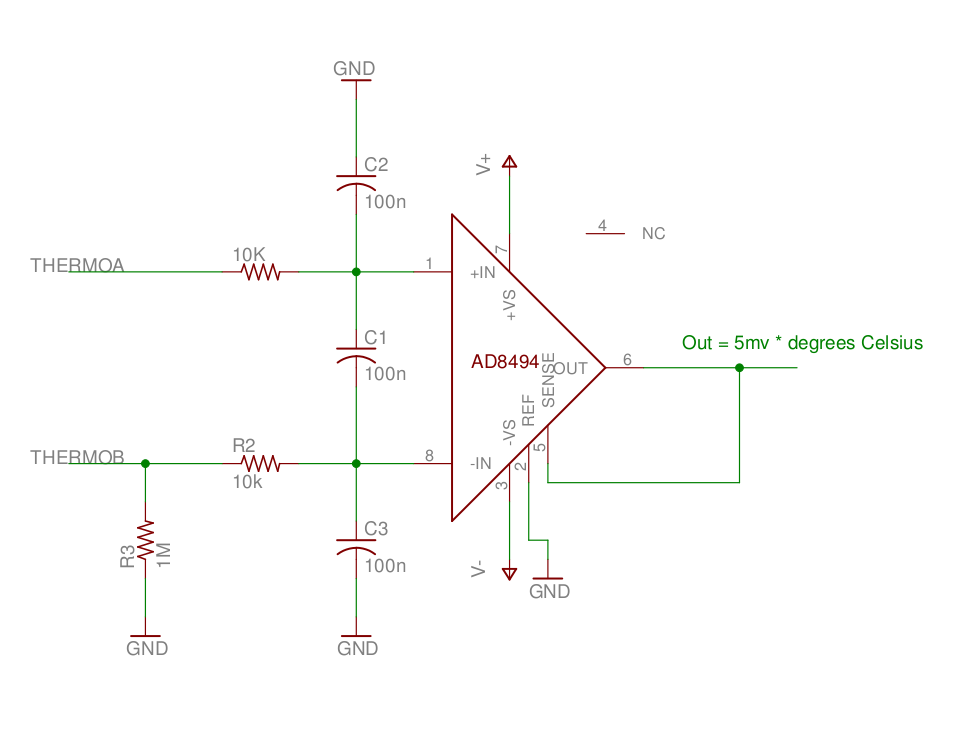
\includegraphics[width=0.5\textwidth]{ThermoAmp}
    \caption{Thermocouple amplifier with 100Hz low-pass filter.}
\end{figure}

Thermal reglation for all heating elements will be handled by toggling a relay
that connects the heating element to the mains. Chilling elements will be
controlled in the same manner, except that the peltier element will be connected
to a 12 volt regulated power supply. This task will be handled by the STM32.
	
All flow monitors will be hall effect based pinweel sensors. These sensors
deliver a series of electrical pulses proportional to the amount of fluid
flowing through them. Timers and interrupts on the STM32 will be used to make
these measurments. 

% TODO Consider revising first sentence to simply ``user data''
% I'm a little confused about whether this is server side to client side -Aaron
\subsection{Data Aggregation and Processing Overview}
The application will store user registrations, favorites, and other data in a
standard SQL database. This database will be hosted separately from the
machine, and could potentially be on a cloud service provider. The server will
be encapsulated in a Wildfly(JBoss) application server implementing the Java
Enterprise Edition Standard. Wildfly provides a container that can manage the
database and its communication with the user application. The REST protocol
will be used to communicate with the Wildfly server. Java code running inside
the Wildfly server will translate JSON objects sent by the user into Java
objects. MyBatis mappers will be used to dynamically translate these objects
into SQL statements to update the database. The database will posses a users,
beverages, and favorite's table. The users table will store core user data:
name, email, salted password hashes, etc. The beverages table will store all of
the settings you would need to instruct the coffee maker to produce an exact
drink. Each beverage and user table row has a unique UUID. Each favorites list
row will be connected to a single user via the UUID. Finally, each row of the
favorites list will store all of the UUIDs that are associated with that list.
That way, when a user sends a REST protocol request to get all of the favorites
list of a particular user, MyBatis can generate a SELECT request to grab all
the relevant lists from the favorites table and then use the uuids stored
within those rows of the favorites table to grab the drinks associated with
each list. All the aggregated data is then returned to the user via REST protocol.

% TODO This section should probably go after the flash section
\subsection{Raspberry Pi Setup and Initialization}
%TODO Actually build up and run http://mattrichardson.com/Raspberry-Pi-Flask/ on a flask server
% and right down the steps for setup. Setup should be very similar


%TODO This is written as if there will be microcontroller in conjunction with
% the RPI. I don't think that will wind up being the case - Aaron
% ADDENDUM I'm starting to think maybe that's not such a bad idea - Aaron
\subsection{Flask}
Flask is a web framework that provides tools to allow you to build a web application.
Flask is a micro-framework, so it requires no outside dependencies or external libraries.
This means that Flask is lightweight. Flask is designed for creating web applications,
with a databse backend that operates through the browser. We will be using it to open
a port on the local wifi network that will act as a REST server. We will use this server to send
commands through the Raspberry Pi to the microcontroller. Thus, Flask is a middleman from the 
android application and the components inside the coffee machine.

\subsection{Mobile Application}
The UI will be implemented as an Android application written in Java. Upon
opening the application, it will ask the user to pair their Android device to
the coffee machine given it's serial number. Afterwards, it will take the user
to a login screen which will allow give the user the option of registering.
Registering and implementing a database is a stretch goal for us, our first priority is a simple UI that functions well with the coffee machine. 

For registration, the idea is that we will allow the user to have a few extra options given from a database
integration. These options will allow the user to search recent beverage
choices, favorites, recommendations, schedules, and an online database. Each
menu will include a similar list layout with searchable drinks. Upon clicking
one of the listed items, it will show all of the settings and have descriptions
based on what the user (whether it is yourself or another user) has written. It
will then have the option of favoriting, brewing, and scheduling the drink
right in that given screen. In the scheduling menu, drink schedules may be
canceled or changed. The benefit of registering will allow a user to login on
any application and have all of the features described above.

Given the choice of not creating a login, which is our base goal, a user will still have to pair their
phone to the device through the database, but won't have to deal with any extra
UI that comes with a registered user. A non-registered user will be allowed to
brew coffee the way they want at that instant. 

For the beverage creation menu, there will be advanced and basic settings options, allowing the user to be very
precise, or general in their brew. Once all settings are selected, if
registered, a user may have the decision to leave information on the drink
created and post it in a searchable database and/or their recents/favorites.
Information may be a title, description, etc. If the user is not registered, it
will not prompt them for anything and brew their drink. 

The mobile application
will have the job of communicating between the FLASK server hosted on the 
Rasperry PI, which in turn controls the coffee machine via GPIO pins. To be
precise, the goal is to create a simple UI that controls the coffee machine the way it should.
If time is generous, we will then try to implement communication with a database and
maybe some more features on the mobile app.


\section{Mobile Application}
In this section the communication between the mobile application and the FLASK
server hosted on the Raspberry PI. The skeleton for the the application itself will
also be discussed, specifying the general layout/functionality of the application, as
well as the stretch goals that we will be implemented if time is generous and things
go smoothly.

\subsection{Communication between FLASK and App}
The machine will be hosting it's own web server that the user application will
be communicating with. It will have a REST API that will allow us to control the
board, and in turn the machine as well. Within the android application itself,
we can use a class called Java.net. Within that class we will be able to use
things such as HttpURLConnection to send HTTP requests such as GET and POST
requests. For Java HTTP GET requests we can get all the info we need in a
browser URL. We can use static functions or functions with parameters within
that URL. An example of a GET request would be something like: \\ \\
\textbf{http://localhost:8080/CoffeeMaker/login?userName=Jim}\\ \\which could
be a request for the user information on a user named "Jim". We could also send
out information in a POST request that would be received on the local server
and then interpret the information and perform an action. There are also other
actions that are useful in REST API's such as PUT, PATCH, and DELETE. Steps
below are ones that would be used to send HTTP requests to the server using the
HttpURLConnection class:
\begin{itemize}
\item Create a URL object with a GET/POST URL string like one mentioned above
\item Open a connection with that URL that creates an instance of an HttpURLConnection
\item Set the request method in the HttpURLConnection
\item Call setRequestProperty() on HttpURLConnection
\item Call getResponseCode() to see if the request was processed successfully or
if there were errors
\item For GET, use a Reader and InputStream and process the response
\item For POST, before reading the response, get an OutputStream from
HttpURLConnection and write POST parameters into it.
\end{itemize} 
\ \\
\textbf{The flask API will expose 3 API calls to the localhost:} \\ 
\begin{itemize}
\item The first API call will be to verify that it is connected, this call will
be a GET call to verify connectivity. If the call succeeds a 200 response will
be posted as well as the session number, UTC timestamp, and model of the
machine in a json formatted payload.
\item The second API call will be to initiate a brewing cycle. This will be a
POST call with machine settings embedded in the url or in a payload sent. If the
call succeeds a 201 response will be posted as well as session number, utc
timestamp, model and the data that was interpreted. If the machine is currently
making a cup of coffee, it will respond with a 200 response that indicates that
the machine is busy and the order will either be queued or discarded.
\item The third API call will be to send the most recent 10-20 requests back in
a json format. This will be a GET call that will tell the Flask server to pull
the latest user data for that machine down, and send it back to the client. If
this succeeds, a 200 Response will be posted as well as a session number, UTC
timestamp, model, and json formatted rows of data about previously made drinks.
\end{itemize}
\ \\

% TODO - Need to improve clarity on these first couple sentences. They're kind
% of hard to understand
The REST API will be exposed to anyone on the network as it will run on host
'0.0.0.0'. '0.0.0.0' is a non-routable address that allows all IPV4 addresses
on the network to be listened to on the Raspberry Pi operating system.
However, each request will not be accepted by the machine unless it has a
serialized key that matches the machine data. Each machine will come with a
unique serial number that must be included in each request in order for the
request to be accepted. This will validate that a request is intentional, and
legitimate.
The flask application will control and log every request made, as well as push
every coffee call up to an external database, making it the only device that is
pushing up to the database.

% TODO Can we add some figures with the UI?
\subsection{UI Skeleton}
For the user interface, we aim to setup something simple for a user, then if we
have more time, we will try to integrate a database into the machine that would
effect the mobile app as well. For the first part of this section, the focus will be
on what we aim to accomplish. The rest of the section will be on the database
stretch goal skeleton. The mobile application will not be too complex and will
probably consist of only a few activities in an Android Application. As usual
for many UI applications, we will be using a Model View Controller (MVC)     
concept.  Android studio can be nice, because it is completely possible to have
the model and controller in one section and the view in XML or another class
file that would most likely implement a canvas. Functionality is the first
objective, so an XML View, and Model/Controller activity class would probably
be the simplest form for a few activities.

\par For the main activity, the idea is to have a very simple main title screen
with a single button. As usual with all widgets, we we have listeners that will
react to an action on them. This button will most likely say "connect", which
will then open a new activity, or if already connected to a device that is
recognized as one of our machines, the application will skip the second
activity and go straight to the brewing portion of our application. 
If the mobile device had never been connected to the machine, the first
activity would take you to the next activity on a "connect" button push that
would let you connect to wireless access points around you (just as you
normally would connect to wifi). The list of wireless access points will most
likely be in a recycler view (basically a scrollable view with multiple
entities) One of those access points will be the Raspberry PI's, and once that
recycler view card is tapped, a listener will fire and highlight the card,
letting the user know which one has been selected. There will also be a "back"
button that will always be usable and a "connect" button that will only be
usable once a card is selected. Once the "connect" button is selected, the
application will send out a request to that access point. If that device is one
of our coffee machines, it will send a specific message that will let the
mobile app know that it is the correct device and open the brewing activity.

\begin{figure}[!ht]
\centering
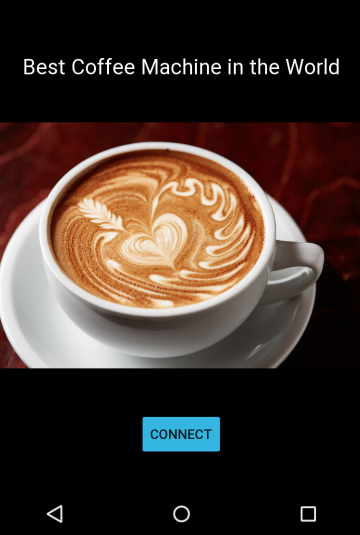
\includegraphics[width=0.4\columnwidth]{connect.png}
\frame{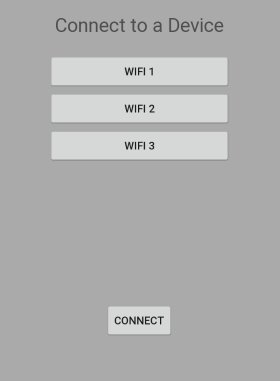
\includegraphics[width=0.4\columnwidth]{wifi.png}}
\caption{Basic mockup of the homescreen, and wifi connection}
\end{figure} 

\par  In the brewing activity there will be many different widgets that control options
on the coffee machine. There are Spinners, Buttons, Sliders, Seekbars, etc. to control
the different mechanisms within the coffee machine. The different
mechanisms that will need control are temperatures of water/milk, PSI values for water/frothing,
amount of milk(ounces), amount of froth(percentage), what kind of syrup and how much, the amount of coffee, and the fineness
of coffee grounds. These will all be represented as integer values. Below is a mockup of the brewing activity:

\begin{figure}[!ht]
\centering
\frame{\includegraphics[width=0.5\columnwidth]{brewNoUser.png}}
\caption{Basic mockup of brew activity}
\end{figure} 

\subsection{Mobile Stretch Goals}
The idea of having a database attached to this whole system is something that we would like to do, but we may not find time.
Depending how much data we would want to keep track of would cost more and more in time.
Ideally we would like to create a system that keeps track of previous drinks, favorited drinks, and create scheduled times for drinks.
The other idea would be to allow a cross integrated system between all users and allow them to share beverage ideas and also
have a feature of recommended drinks.

\par If we were to implement this, when opening the application, instead of directly going into connecting with a device, we would
have the option for the user to login or continue without logging in. If the user didn't have an account they could create one by
giving an email, login name, etc. They would then have to verify their email before continuing. The way we could go about doing this 
is by using Firebase. Firebase is a google database, we would implement the Raspberry PI to communicate with Firebase and then
relay the data back to the mobile devices attached. On the mobile side we would send http requests to the Raspberry PI to see
if the user existed or not and login using that information. It is also very possible to do Bluetooth communication with the Raspberry Pi
and mobile application and have the mobile application just use cellular or wifi to communicate with the Firebase server. For right
now we are aiming at using the Raspberry Pi as the center control for everything.

\par If the user had not logged in, the the previous ideas mentioned before would be presented. If they did login, they would be 
presented with a menu with multiple options. Those options would be the ones that were listed before: Recent Drinks, Favorited Drinks,
Scheduled drinks, Recommended drinks, and searchable drinks. If anything the first stretch goal would be to get Recent, Favorited, and Scheduled
drinks implemented, because that does not require cross data integration between other users. Integrating the database would allow users to login
with different devices on different coffee machines and have their own data readily available to them.

\par Drink brewing would be a little bit different for users. Upon creating a drink, it would allow you to upload it to the database or add it to your favorites; also allowing the user to  add a description of it,
allowing other users to search for it in the other "search" menu. This option would be available when pushing the button to "brew" your drink, a popup would display, having a textbox for description, spinners
for times, check marks to enable things like setting schedules or uploading to the database or adding to your favorites list. Same concept of brewing, but with added features to save data for the user.

\par Opening the recent menu would display a view that had the last few drinks you had brewed. The drinks would probably be listed as as some sort of card (object that holds info) and
upon clicking the card, it would bring up the brewing menu but, but the one like the one listed in the above paragraph; performing the exact same way.

\par Opening the favorited menu would be a little like the recent menu, but most likely be in a recycler view (a view that holds cards and is scrollable). The cards would act the exact same way
as the other cards in the previous sections, opening the brewing action. The difference with this menu is that the user would be allowed to remove favorited items. There would most likely be
a check mark next to all of the cards and once selected, a button would highlight that would allow you to delete it; perhaps even editing could be implemented as well.

\par The scheduled menu would be the exact same layout as the favorited menu, but it would allow you to edit as well, setting times to how you want them. There would probably be
a new type of action that would be made specifically for this. Opening a popup specific to changing times on a specific drink. There would be spinners and and check marks, allowing
users to make recurring drink schedules or a one time schedule.

\par Recommended and Searchable features are ones that would require data aggregation. The recommendation menu would be laid out the same as the others menus. It could either 
have a set limit of recommended brews (preferably easier) or a scrollable list that updates as it goes (probably not ideal for this project). The functionality would be the same, by clicking on
a card, it would take the user to the brewing screen where they could make it a favorite, brew it, etc. Some sort of user cross referencing algorithm would have to be used to select data
from the database for recommended brews. A simple query could probably be used for that, but it is possible to create something more thorough. The searchable feature would require
some sort of search box, and implement a query based on that search box. These queries would be executed by the Raspberry Pi and sent back to the mobile application, the app would
just need to send queries through http calls.
Since there probably would not be very many tables, the searching would not be too hard to implement. These
two would be the most difficult to implement out of the features in this stretch goal. \\ Figure 4 shows some mockups of user
features; Figure 5 shows some other user activities that would be used.

\begin{figure}[!ht]
\centering
\frame{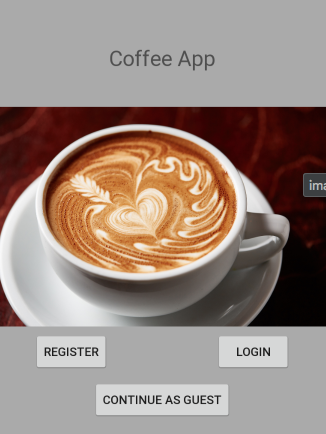
\includegraphics[width=0.4\columnwidth]{loginStretch.png}}
\frame{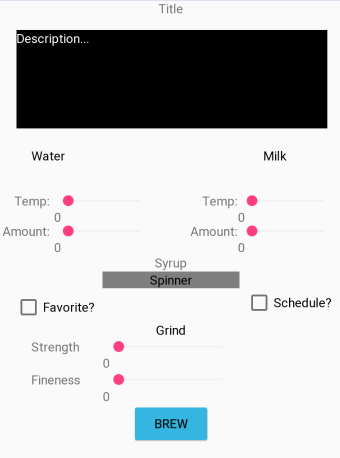
\includegraphics[width=0.4\columnwidth]{brewStretch.png}}
\frame{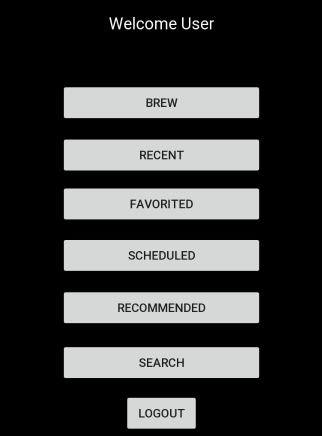
\includegraphics[width=0.4\columnwidth]{menu.png}}

\caption{Basic mockup of user login, brew, and menu screens}
\end{figure} 

\par
\begin{figure}[!ht]
\centering
\frame{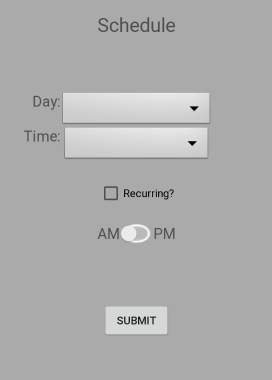
\includegraphics[width=0.3\columnwidth]{Schedule.png}}
\frame{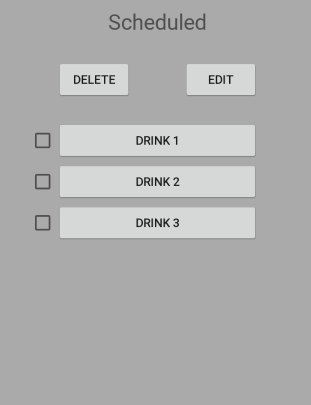
\includegraphics[width=0.3\columnwidth]{Scheduled.png}}
\frame{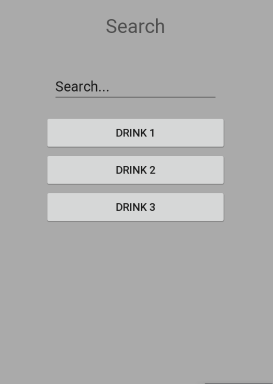
\includegraphics[width=0.3\columnwidth]{Search.png}}
\frame{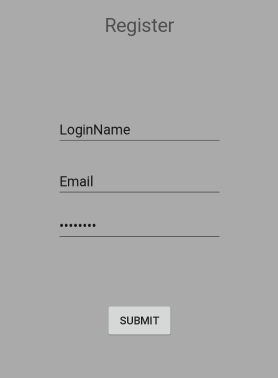
\includegraphics[width=0.3\columnwidth]{Register.png}}
\frame{
\includegraphics[width=0.3\columnwidth]{Load.png}}
\caption{Basic mockup of other screens such as: Creating schedules, searching, Registering, and a schedule screen, and waiting for email confirmation}
\end{figure} 

%\subsection{Data Aggregation and Processing Overview}
% The application will store user registrations, favorites, and other data in a standard SQL database. This database may be hosted separately from the machine, and could potentially be on a cloud service provider. The server will be encapsulated in an application server. The application server provides a container that can manage the database and its communication with the user application. The REST protocol will be used to communicate with the application server. Code running inside the application server will translate JSON or XML objects sent by the user into Java objects. Mappers will be used to dynamically translate these objects into SQL statements to update the database. The database will posses a users, beverages, and favorite's table. The users table will store core user data: name, email, salted password hashes, etc. The beverages table will store all of the settings you would need to instruct the coffee maker to produce an exact drink. Each beverage and user table row has a unique UUID. Each favorites list row will be connected to a single user via the UUID. Finally, each row of the favorites list will store all of the UUIDs that are associated with that list. That way, when a user sends a REST protocol request to get all of the favorites list of a particular user, the mapper can generate a SELECT request to grab all the relevant lists from the favorites table and then use the uuids stored within those rows of the favorites table to grab the drinks associated with each list. All the aggregated data is then returned to the user via REST protocol. 
%The application will store machine data, and individual coffee customizations in a standard SQL database. 
%The database will be hosted on a cloud service provider (AmazonS3 or Firebase). Each machine will have it's own table for statistics on its own components to document wear and usage. 
%Coffee customizations will be in a global database table where it will store information about the individual customizations of the cup of coffee as well as the serialized number for the coffee machine, for
%ease in sorting through machine by machine usage.

\section{Database Integration}
(Stretch Goal) Our goal for the DB integration is to used a free DB hosting service such as AWS or Firebase
to accumulate data about recent machine requests and generic machine usage statistics. Machine requests will
be sent in as a json object, and will likely be represented in the DB as a json object. The goal for collecting request
data is to for the user to have a history definition for tweaking and repeating, and for us to aggregate what common 
settings are for future optimization. Each request will be held in a global database, with a unique machine specific
key for querying a specific machine only. The machine statistics are meant for durability data, and to analyze data in hopes for future optimization.
Machine statistics will not be kept in a global table, and are only meant for local use.

\section{Project Tasks}
\subsection{Flask}
\begin{itemize}
\item Flask running on Raspberry Pi
\item Flask running on startup and reboot
\item Flask connected call
\item Flask control of inner components
\item Flask Coffee Call
\item Flask DB Connection (Stretch)
\item Flask DB Push (Stretch)
\item Flask DB Pull and Return on Call (Stretch)
\end{itemize}
\subsection{Database Integration (Stretch Goal)}
\begin{itemize}
\item AWS or Firebase Setup
\item Setup Request Global table
\item Setup / Test push \& pull to request table
\item Setup Local table
\item Return only machine specific data
\end{itemize}


\subsection{Physical Machine}

\begin{itemize}
\item Design frothing mechanism
\item Design tamping mechanism
\item Burr design completed
\item Design temperature regulation circuity
\item Design mainboard based around the Raspberry Pi Compute Module
\item Design grinding mechanism
\item Fabricate frothing wand, tamping mechanism, and burr plate mold
\item Fabricate ceramic burr plates
\item Construct boilers
\item Construct refrigeration system
\item Assemble grinder
\item Assemble brewing system
\item Assemble frother
\end{itemize}

\subsection{Mobile User Interface}
\begin{itemize}
  \item Login screen which allows optional user login/registration or not.
  \item Device pairing screen
  \item Beverage creation screen has an advanced/basic toggle button and sliders, value inputs, and other selections
  \item Communication between application and FLASK server.
  \item Recommendations, scheduling, recents, favorites, and search sharing same UI layout, some using database(stretch goal).
\end{itemize}

% Just guessing here, but in an ideal world this would be the waterfall outward
% Inidividual Components working
% Components Controlled By I2C -> Aaron: At the end of the day, everything will
% be controlled by I2C or SPI
% Components Controlled via USART Serial -> Aaron: unlikely, except for possibly
% a debugging interface
% Components Controlled via Flask API Calls
% Flush out Flask buffer and all calls
%% We probably need a buffering system since the machine throughput will be low
% Flask talking to DB
% Flask talking to Android Device
% DB Pushing valuable data downstream
%Machine talking to Android Device
\subsection{Machine Side Software}
\begin{itemize}
  \item Flask application setup
  \item Flask can receive commands from Android application
  \item Mainboard communicating with regulators and monitors
  \item Mainboard controls motors, servos, and steppers
  \item Mainboard can adjust grinder fineness and start/stop grinding mechanism
  \item Mainboard can initiate tamping process
  \item Mainboard can initiate brewing process
  \item Mainboard can initiate frothing process
  \item Mainboard can initiate cleaning process
\end{itemize}

\subsection{Database/Web Server}
\begin{itemize}
\item Decide which application server, database mapper, and programming language to use for web server.
\item Setup application server that is capable of receiving and sending REST requests.
\item Establish API for communicating with android application (decide on communication format, i.e. xml or json)
\item Convert REST data into language specific objects. 
\item Develop a set of mappers that can convert language specific objects to SQL inserts and vice versa.
\item Set up SQL Database and populate schema. 
\end{itemize}

% Leave this to me - Aaron
\section{Project Materials}
\begin{itemize}
\item Raspberry Pi compute module
\item Stainless steel stock
\item Cartridge heaters
\item Custom PCBs
\item Various IC's and discretes % TODO Add more specificity
\item Copper pipe
\item Silicone Tubing
\item Custom machined parts
\item Boron carbide powder
\item PLA plastic
\item SLA Resin
\item Peltier elements
\item Moldmax 30 silicone
\item Servos
\item Stepper motors
\item Peristaltic pumps
\item Thermocouples
\item Liquid pressure sensors
\item DC motors
\end{itemize}

% Raspberry Pi -> compute module, specifically
%Boilers -> Built from raw materials, stainless steel
%Coils -> Cartridge heaters
%Reservoirs -> Built from raw materials, stainless steel or aluminum
%Custom PCBS
%Various ICs and discretes
% Copper or brass pipes or silicone tubing
% Custom machined pieces from proto labs

\section{Testing Approach}

\subsection{Machine Side Software Testing}
% Flask
Testing against the Flask microframework part of our project will be heavily reliant on 'mocking'
outputs and inputs of recieved calls. Flask as a microframework does not need to be tested, however
our devices reaction to GPIO eventst needs to be tested. This can be occumplished using the python
unittest.mock framework  \cite{mock} where we can create tests that will 'mock' returned data to
be able to flush out multiple tests without relying on any network or GPIO setup. We will also have to 
test a buffer system to make sure 'real' requests are getting recieved and queued and multiple requests
of the same requests are discarded.

\subsection{Physical Machine Testing}

\subsection{Mobile User Interface Testing}
Mobile Interface testing will be done one task at a time. Creating the layout and listeners will be the first
 goal. By doing this it will ensure a skeleton to work with. Each screen will be done one at a time,
moving in the flow as a user would. Afterward another pass will be taken, adding data. Starting with the
 login screen, communication between database, webserver, and the device will be established and
  pairing/login data will be tested and verified on every side. We then move to the basic function of non
  registered user: creating a drink. If the mechanical portions are not ready yet, then data collection will
   be done next on all of the other menus: scheduling, favorites, recommendations, recents, and online
    searching. During all of these integrations, testing with the actual coffee machine will take place, 
    ensuring communication is working on all ends. 

% This needn't be more than a paragraph or two - Aaron
\section{Project Demonstration}
At the project demonstration, the machine will be setup with an Android tablet and loaded with ingredients.
Visitors will be invited to use the tablet to design a drink watch the machine
in action. Various spare internal components will be set out to aide in explaining how the machine works.

% Don't think this section is necessary - Aaron
\subsection{Mobile Demonstration}
We will first demonstrate functionality with non registered user implementation (the basics on mobile)
 and how the mobile device can communicate with the machine properly to make a cup of coffee that is
  asked for. Then we will demonstrate how data collection offers different options to users. Grabbing 
  information from the database and laying it out in multiple menu's will give users the ease of quickly 
  making what they need or searching for something new. Using these different menu's, we will show 
  that the data integrity holds and creates the drink as it should. 

\section{Contigency Plans}
\subsection{Flask and Database}
In the case that we cannot complete the project the database element will be scratched. This would affect
Flask part of the project such that the expectation of data pushing and pulling will not be implemented.
If time does not permit us to complete the database section in whole, then the database loses all 
of its importance to this project and thus should not be attempted.

In the case that we cannot demonstrate our project at the University of Utah due to network protections,
we would buy / bring a popup wifi-network that we could connect to.
 

% \begin{thebibliography}{1}
% 
% \bibitem{IEEEhowto:kopka
% H.~Kopka and P.~W. Daly, \emph{A Guide to \LaTeX}, 3rd~ed.\hskip 1em plus
%   0.5em minus 0.4em\relax Harlow, England: Addison-Wesley, 1999.
% 
% \end{thebibliography}

\bibliography{biblio}{}
\bibliographystyle{plain}

\end{document}
\end
